\section{Существующие решения}
\subsection*{GnuCash}

\textbf{Тип}: персональная бухгалтерская система\\
\textbf{Автор}: Robin Clark - X-Accountant,
Gnumatic (Linas Veptas)\\
\textbf{Разработчики}: GnuCash development team\\
\textbf{Язык программирования}: C, Scheme и Java\\
\textbf{Интерфейс}: 	GTK+\\
\textbf{Операционная система}: GNU, GNU/Linux, FreeBSD, macOS, Microsoft Windows и Android\\
\textbf{Первый выпуск}: 1998\\
\textbf{Лицензия}: 	GNU GPL 2\\

\begin{figure}[H]
	\centering
	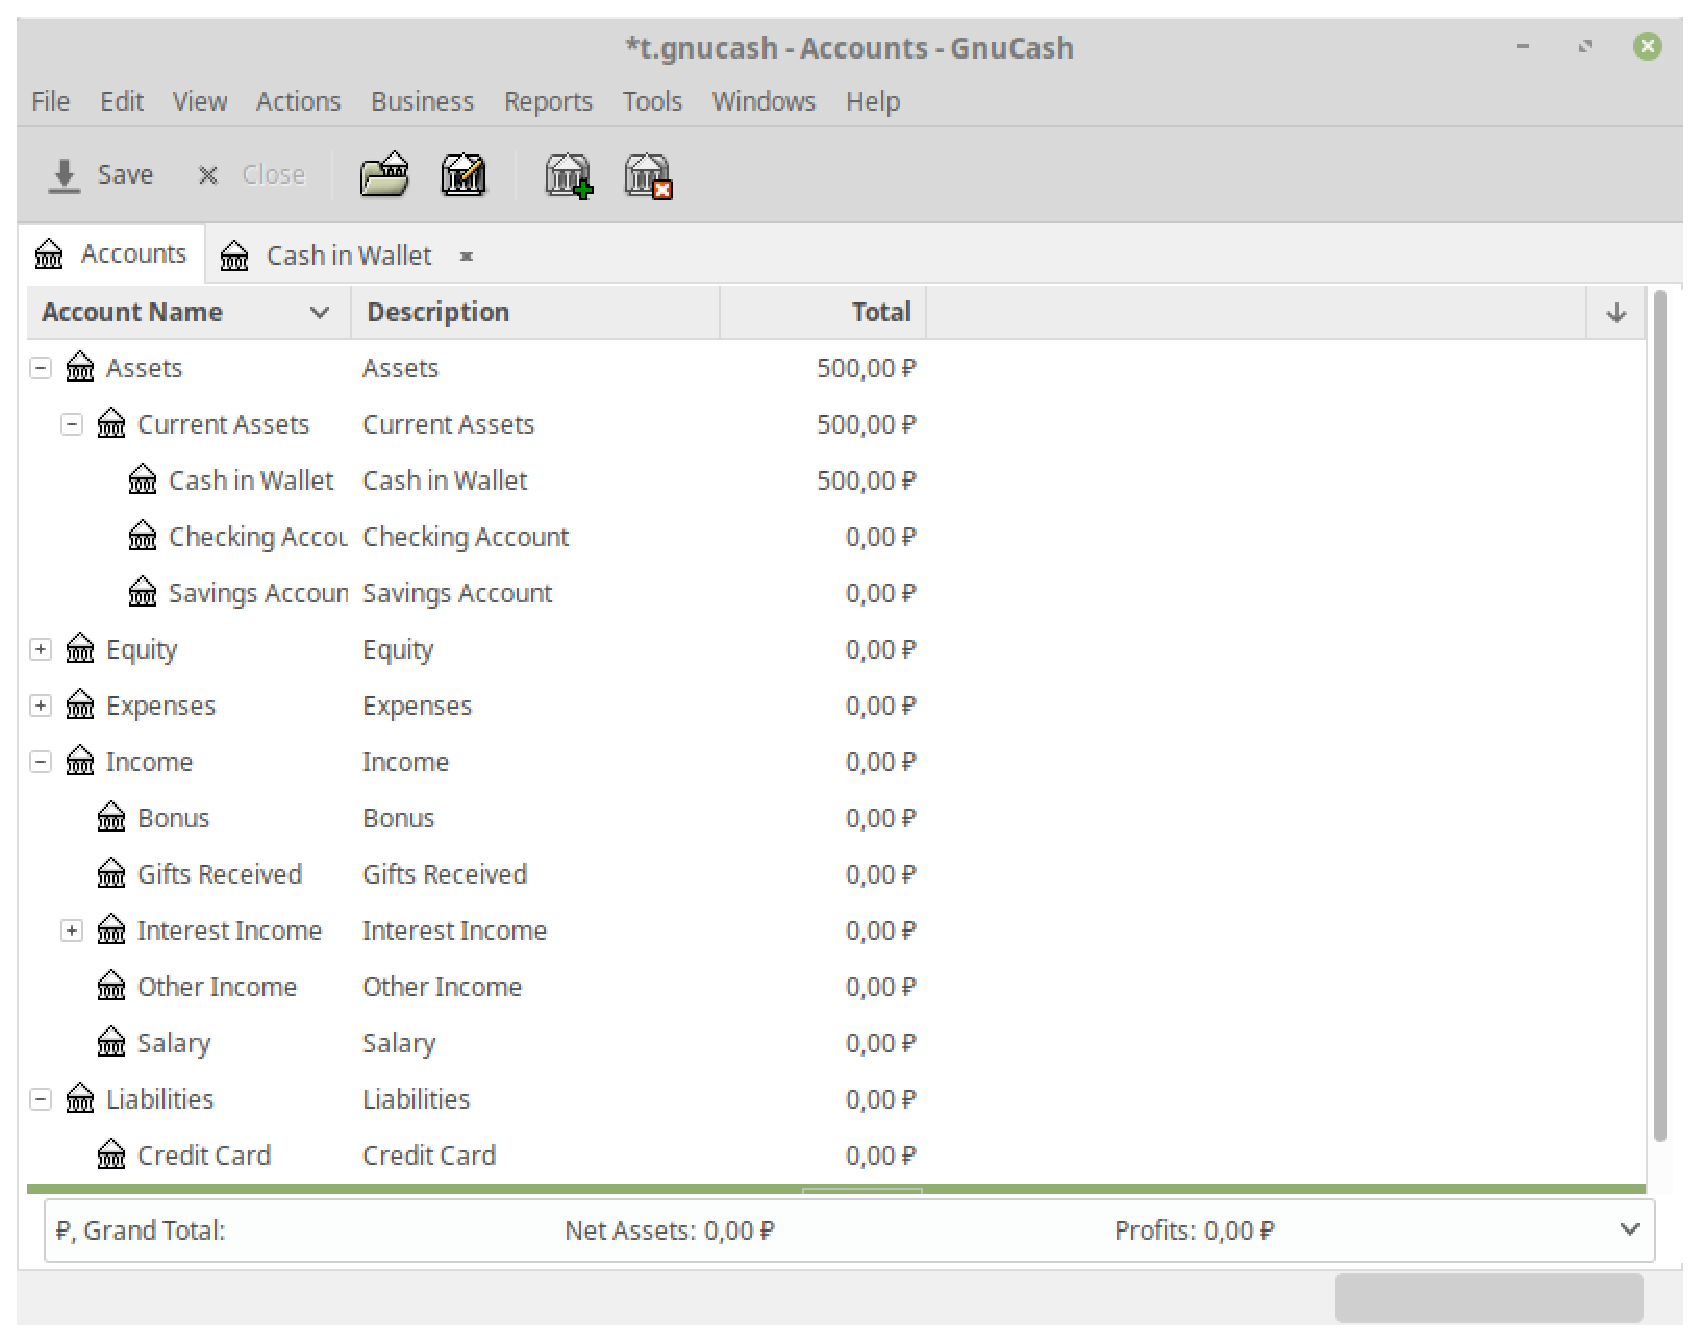
\includegraphics[width=1\linewidth]{pics/GnuCash.eps}
	\caption{Интерфейс GnuCash}
	\label{fig:GnuCash}
\end{figure}

Один из самых известных проектов в мире персональных финансов. Разрабатывается с 1997 года как продукт с отрытым исходным кодом.\\

При переходе на эту программу с других проектов могут возникнуть сложности, т.к. принципы работы GnuCash основаны на системе с двойной записью, характерно скорее для профессиональных платформ бухгалтерского учета. Однако хорошо организованная документация на разных языках (русский есть) и хорошая поддержка помогут быстро разобраться.\\

Почти все свойства программы в сравнении с другими продуктами заслуживают максимальной оценки. Программа продуманна в мельчайших деталях. Способна учитывать различные типы инвестиций, включая драгоценные металлы, ценные бумаги, котирующиеся на наиболее известных биржах (ММВБ нет). Алгоритмизация учета кредитов и других видов долга также на высоком уровне. Среди всех проектов из нашего обзора GnuCash имеет саму продуманную и гибкую систему анализа данных с многочисленными настройками (некоторые из функций анализа есть и в мобильном приложении).\\

Среди слабых мест – ее несколько устаревший интерфейс. Однако он вполне удобен и функционален. При знакомстве с GnuCash становится понятным, откуда многие другие проекты «позаимствовали» основные идеи.\\

Другим очевидным минусом являются минималистичные возможности по синхронизации данных. Предусмотрена только полуручная синхронизация через Google Drive и DropBox, что подходит не для всех. Из этого минуса вытекает и следующий – многопользовательского режима в программе просто нет.\\
Функциональные возможности:\\
\begin{enumerate}
\item Графический интерфейс пользователя
\item Стандартная двойная запись для ведения бухгалтерского учёта
\item Транзакции по расписанию
\item Учёт кредитных платежей
\item Построение отчётов и графиков
\item Поддержка бухгалтерского учёта для малых предприятий
\item Импорт файлов данных из других финансовых систем OFX, QIF
\item (Ограниченная) поддержка многопользовательского интерфейса баз данных SQL
\item Многовалютный учёт
\item Работа с портфелем акций и паями паевых инвестиционных фондов
\item Получение данных об акциях и паях через интернет
\item Финансовый калькулятор
\end{enumerate}
\textbf{Плюс}: Распространяется бесплатно, предусмотрены многие профессиональные функции бухгалтерского учета, возможность ведения управленческого учета для малого бизнеса, постоянное развитие проекта.\\
\textbf{Минус}:Несколько сложна в освоении, принципы работы программы значительно отличаются от большинства других проектов, несколько устаревший интерфейс, отсутствие полноценной синхронизации и многопользовательских возможностей.\\

\subsection*{Streege}
\begin{figure}[H]
	\centering
	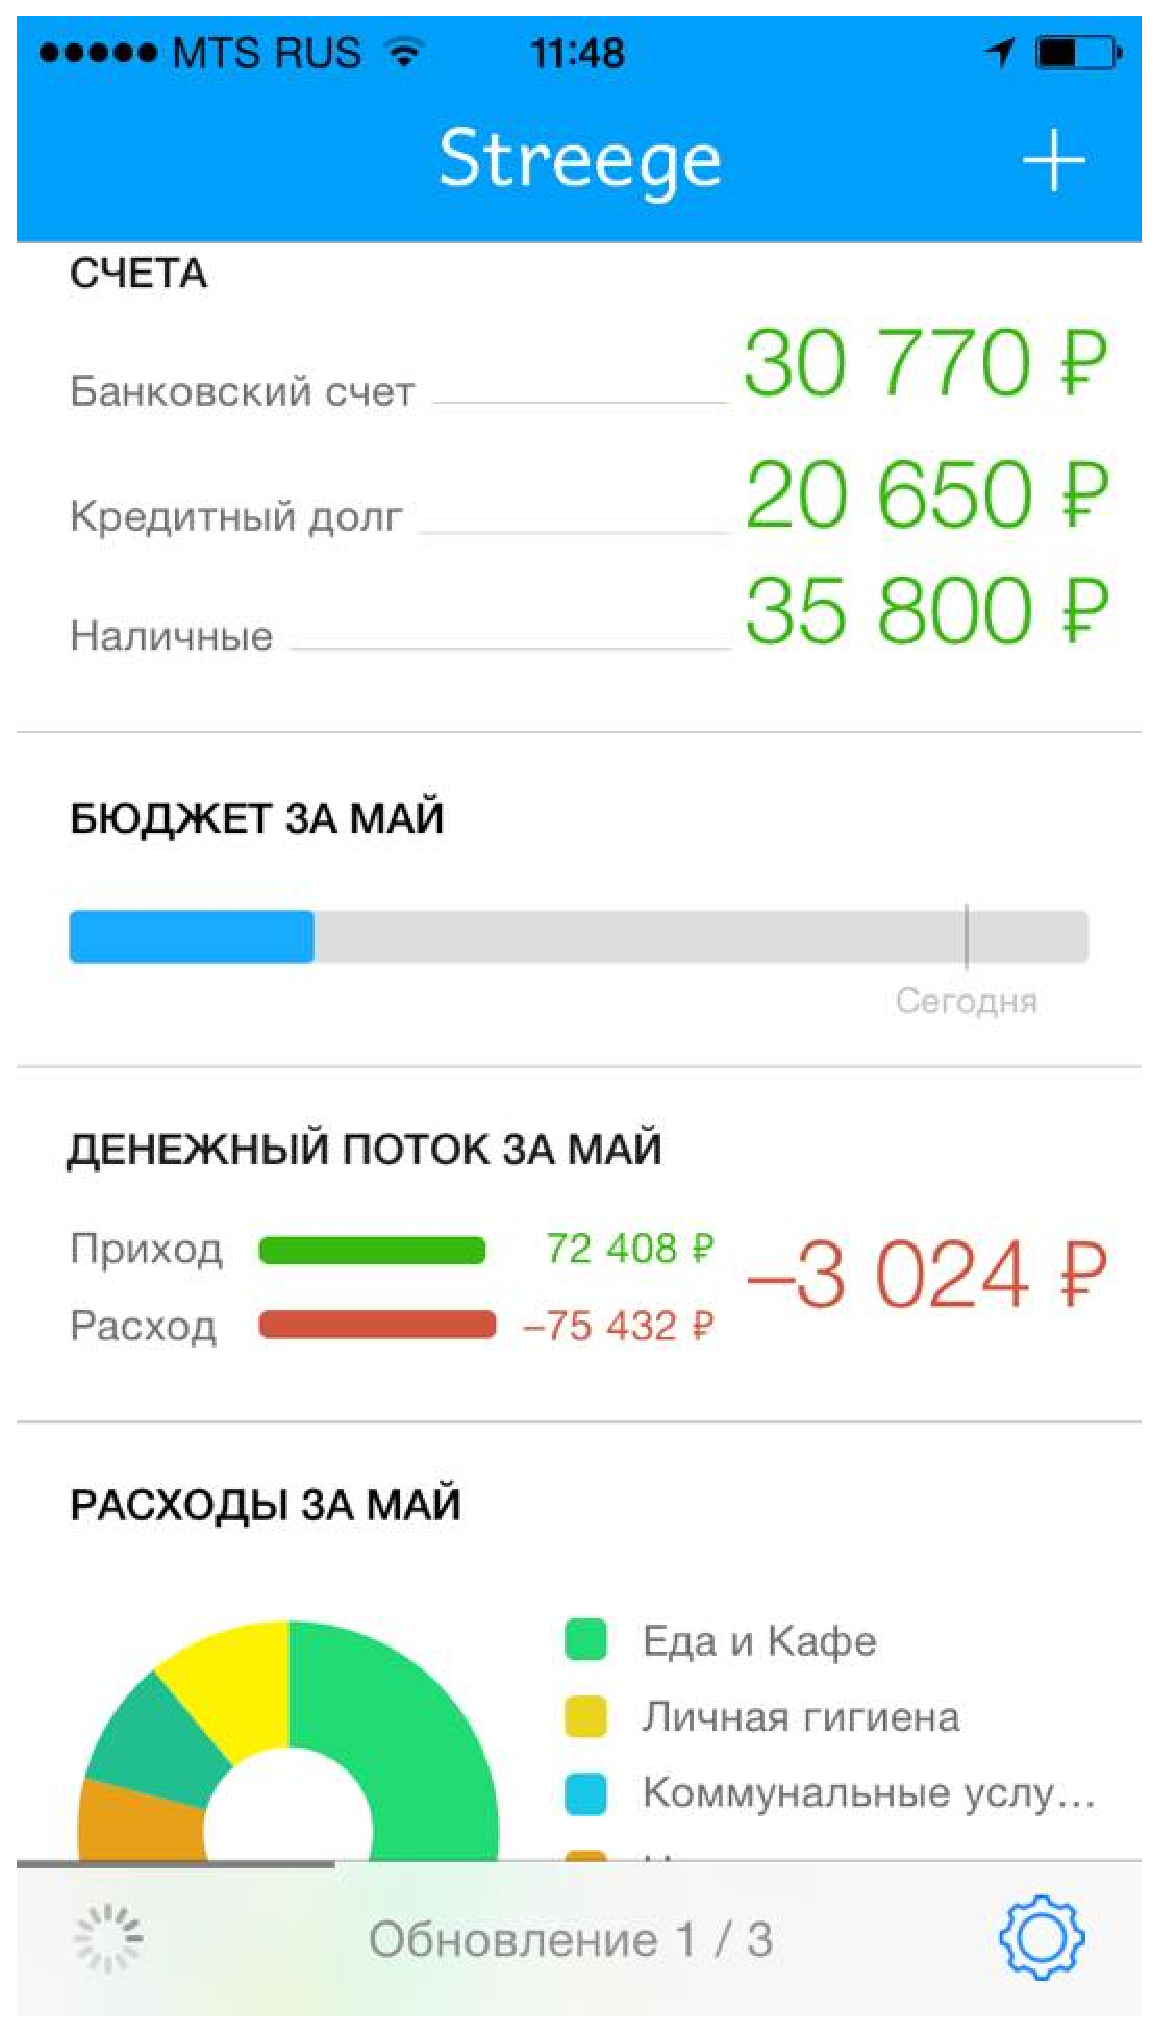
\includegraphics[width=0.7\linewidth]{pics/Streege.eps}
	\caption{Интерфейс Streege}
	\label{fig:Streege}
\end{figure}
Проект запущен авторами CashOrganizer в 2014 году. Это первая на российском рынке программа, которая умеет в автоматическом режиме (без использования СМС и email) синхронизироваться с банками и загружать данные о транзакциях и балансах счетов. Категории платежей так же присваиваются автоматически. Впрочем, все данные платежа после загрузки могут быть отредактированы вручную.\\

Концепция проекта очень удобна для повседневного использования. «Руками» нужно вносить только транзакции из наличных. В перечне уже 177 основных российских банков. Для синхронизации с некоторыми из них (Сбербанк, ТКС и другие) требуется вводить код, высылаемый по смс. Другие (Авангард, Альфа Банк и др.) работают без всяких подтверждений. Но даже введение раз в несколько дней кода из СМС особых проблем не вызывает.\\

Пока в проекте нет онлайн синхронизации, нет сплита транзакций и еще некоторых мелочей. Но проект развивается довольно быстро. Надеемся на исправления всех недочетов.\\

Кроме того, надо конечно понимать, что как у всех проектов, нацеленных на мобильные платформы, возможности для анализа данных и другие продвинутые функций здесь будут ограничены по определению. К сожалению информации по этому продукту очень немного\\
\textbf{Плюс}: Автоматическая система загрузки транзакций из банков. Автоматическое присвоение категорий транзакциям.
\\
\textbf{Минус}:Нет синхронизации.\\

\subsection{MoneyWiz}
\begin{figure}[H]
	\centering
	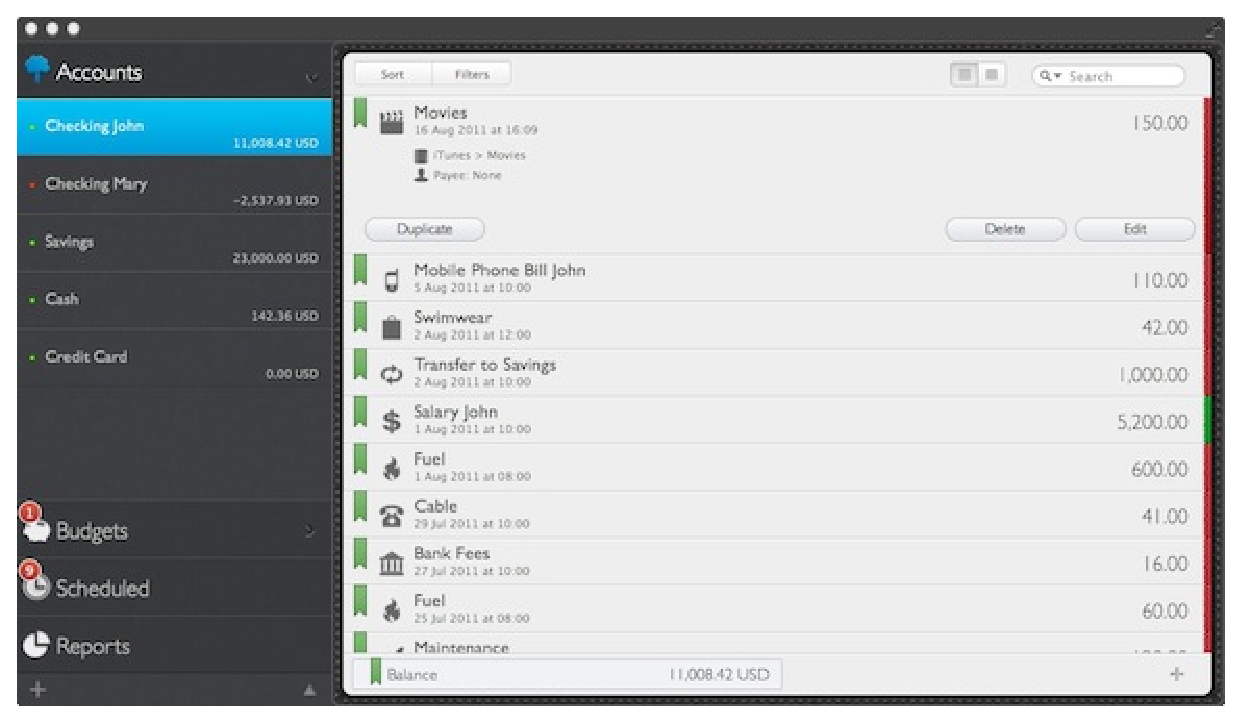
\includegraphics[width=1\linewidth]{pics/MoneyWiz.eps}
	\caption{Интерфейс MoneyWiz}
	\label{fig:MoneyWiz}
\end{figure}
Проект существует с 2011 года и был разработан с прицелом на iPad. MoneyWiz и сейчас остается сервисом с наибольшим количеством возможностей для пользователей устройств Apple. Только для MacOS есть десктоп версия. Хотя на сайте проекта уже анонсирована версия под Windows.\\

Из полезных и оригинальных функций – возможность настройки представления окна ввода транзакций. Это окно используется чаще всего в любой программе, и возможность его настройки «под себя» сильно упрощает жизнь.\\

В проекте много функций, которые сделаны специально для пользователей Apple. В iOS версии есть поддержка Touch ID и экспорта через AirDrop. Есть специальная версия программы для Apple Watch.\\

Удивительно хорошей проработкой, особенно для мобильного приложения, порадовали отчеты с довольно удобными настройками.\\

Из грустного – главный плюс программы, а именно автоматическая синхронизация транзакций с банками, работает пока не всегда корректно. Команда сайта rostber.ru протестировала работу с четырьмя российскими банками. Банк Авангард – всё работает нормально. Альфа банк – настроить не получилось. Сбербанк – транзакции загружаются нормально, но баланс отображается неправильно. Тинькофф банк – транзакции загружаются нормально, но баланс отображается неправильно. Пока такие результаты синхронизации вряд ли можно считать приемлемыми, особенно для платного сервиса (примерно 300 руб в месяц). Хотя не приходится сомневаться, что по примеру проекта Стриж, сервис удастся довести до нормальных результатов. Пока MoneyWiz – это единственный проект, где синхронизация транзакций заявлена как для зарубежных и российских банков. Всего проект поддерживает синхронизацию с 15 тыс. банками из 43 стран.\\

Другим явным недостатком является отсутствие колонки (или итога по дням) для баланса счета в перечне транзакций. Во всех продвинутых программах этого уровня балансы ужа давно интегрированы и значительно упрощают жизнь.\\

Странным показалось, что при возможности формирования неограниченного числа бюджетов нельзя включать в них доходные категории (только расходы).\\

MoneyWiz известен, как проект одним из первых в мире (если не первый) проектов в области личных финансов, запустивший синхронизацию данных через облачный сервис. Это случилось в 2011 году. Жаль, что с тех пор мало что изменилось. Синхронизация данных возможна только через непонятный SYNCbits, где необходимо создать учетную запись.\\

Описание функций программ есть только на сайте и только на английском. Каких-либо обучающих материалов не предусмотрено.\\

\textbf{Плюс}: Автоматическая синхронизация транзакций с российскими и западными банками.
\\
\textbf{Минус}:Ошибки в синхронизации транзакций с банками.\\
\textbf{Минус}:Сравнительно высокая стоимость.\\

\section{Разработка собственного програмного обеспечения для учета семейного бюджета}

Как правило систематическое занесение доходов и расходов в таблицу, а
также подсчет итогового баланса может оказаться весьма непростым занятием, но и использование электронных таблиц и специализированных программ
тоже не тривиальная задача, поскольку такие методы разрабатываются с учетом максимально широких возможностей использования, от самых простых
табличных расчетов и до учета дивидендов от приобретенных акций, что не
очень хорошо ложится на базовый семейный бюджет.

\subsection{Выбор языка программирования}

Поэтому я и решился на разработку своего приложения, которое будет
максимально комфортным в использовании и обладать набором функций,
которые необходимы мне,не очень сильно использовать ресурсы компьютера.
При выборе языка программирования для создания приложения я остановился на трех базовых концепциях:

\begin{enumerate}
\item Портируемость
\item Легкость
\item Удобство использования
\item Большие возможности
\end{enumerate}

Благодаря этому списку мне удалось достаточно сильно сократить число
языков программирования на которых можно было написать приложение, в
итоге я остановился на языке

C++ с расширением QT Framework. Который оказался достаточно комфортным и легко расширяемым для выполнения необходимых задач.

\subsection{Разработка базовой концепции приложения}
В качестве базовой концепции приложения был выбран вариант модифицированных электронных таблиц. Самым простым вариантом была следующая структура
\begin{enumerate}
\item Размер операции
\item "Сторона"операции (приход/расход)
\item Коментарий к операции
\item Дата и время операции
\end{enumerate}

Остаток вычислялся путем последовательного суммирования (с модификатором "стороны") размеров операции отсортированных по датам и времени
операции

\subsubsection{Начало разработки}
Первоначальная версия сущестовала в консольном виде без взаимодействия с курсором мыши. Данные хранились в текстовом виде, что позволяло
легко модифицировать записанные данные. Позже были добавлены категории записей, которые позволили однозначно делать подсчет расходов по категориям расходов.

\subsection{Разработка графической версии}
Немного позже был разработан первоначальный вариант графической версии приложения, он по прежнему записывал данные в файл и при этом работал достаточно неэффективно.

\begin{figure}[H]
	\centering
	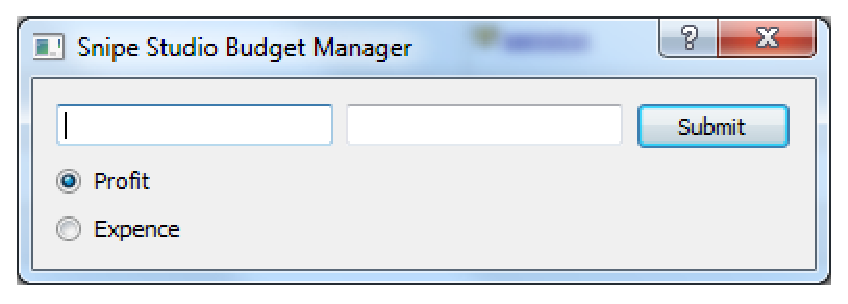
\includegraphics[width=0.7\linewidth]{pics/firstVersion.eps}
	\caption{Первоначальный вариант графического приложения Budget Manager}
	\label{fig:firstVersion}
\end{figure}

Немного позднее было добавлено поле отображающее список операций

\begin{figure}[H]
	\centering
	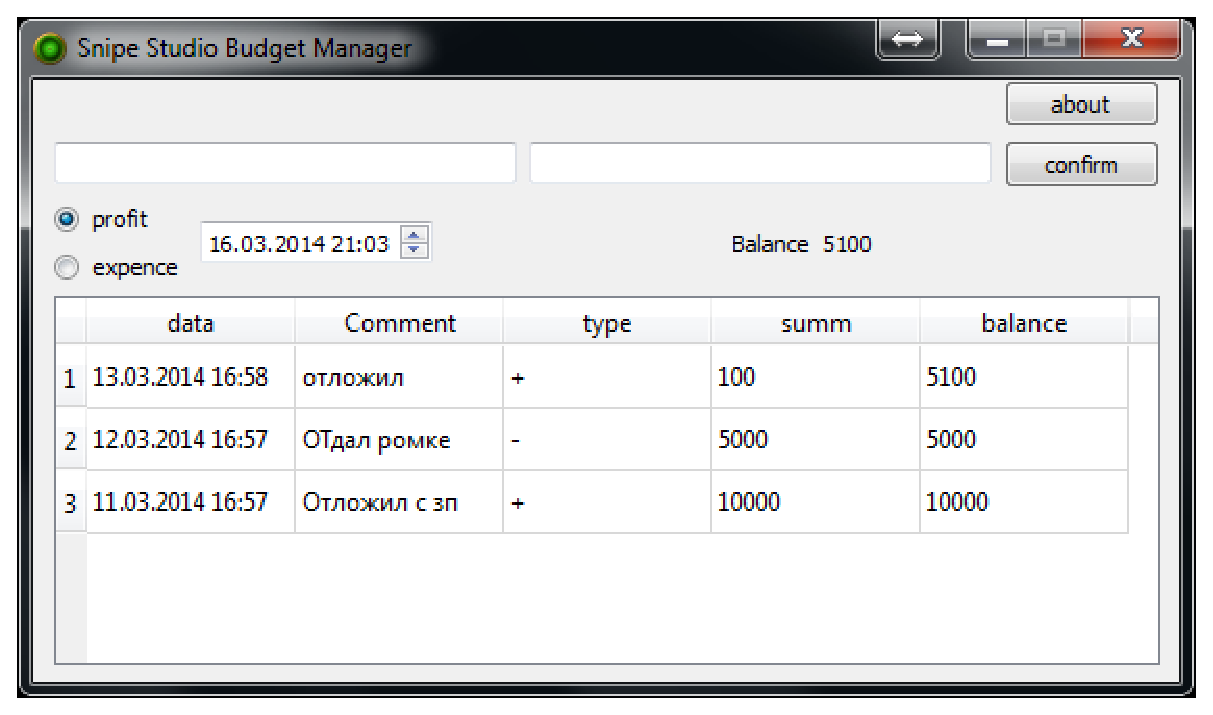
\includegraphics[width=0.7\linewidth]{pics/secondVersion.eps}
	\caption{Вариант графического приложения Budget Manager с таблицей со списком
операции}
	\label{fig:secondVersion}
\end{figure}

Дальше был изменен метод хранения и изменения уже существующих записей, добавлено полноценное меню настроек, строки таблицы теперь окрашиваются в зависимости от выбраной "стороны"(приход/расход) для операции

\begin{figure}[H]
	\centering
	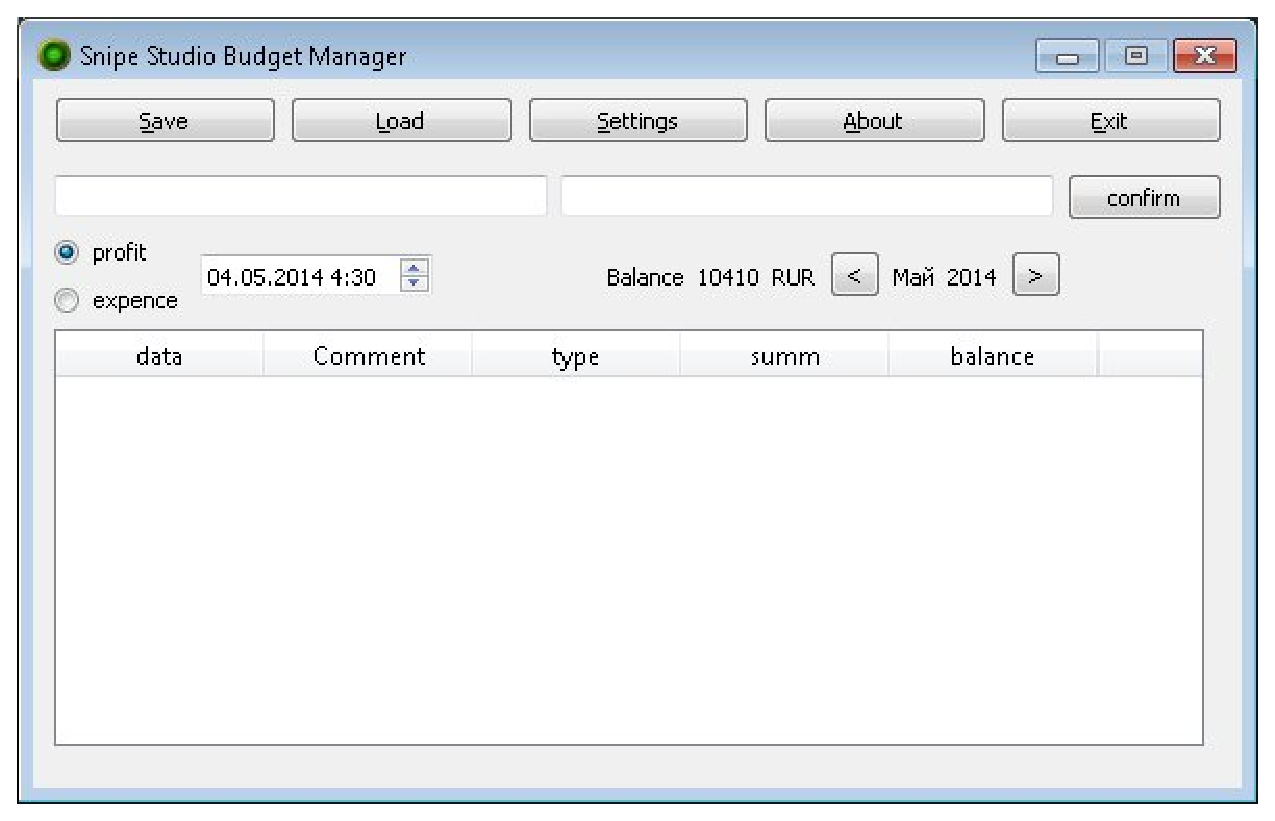
\includegraphics[width=0.7\linewidth]{pics/view1.eps}
	\caption{Окончательный вариант графического приложения Budget Manager}
	\label{fig:view1}
\end{figure}

Позже был изменен общий графический дизайн приложения 	и стал следующим:

\begin{figure}[H]
	\centering
	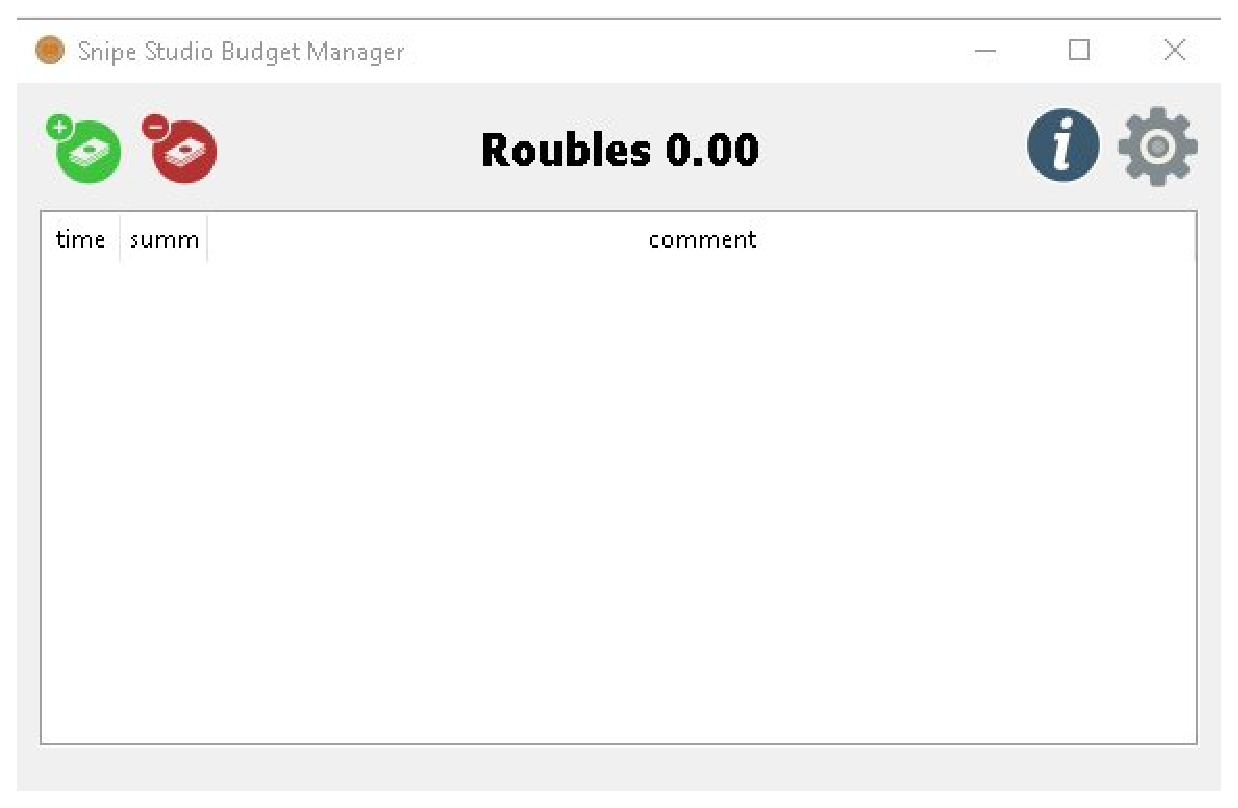
\includegraphics[width=0.7\linewidth]{pics/view2.eps}
	\caption{Второй вариант графического приложения Budget Manager}
	\label{fig:view2}
\end{figure}

Так же была собрана версия для Android

\begin{figure}[H]
	\centering
	
	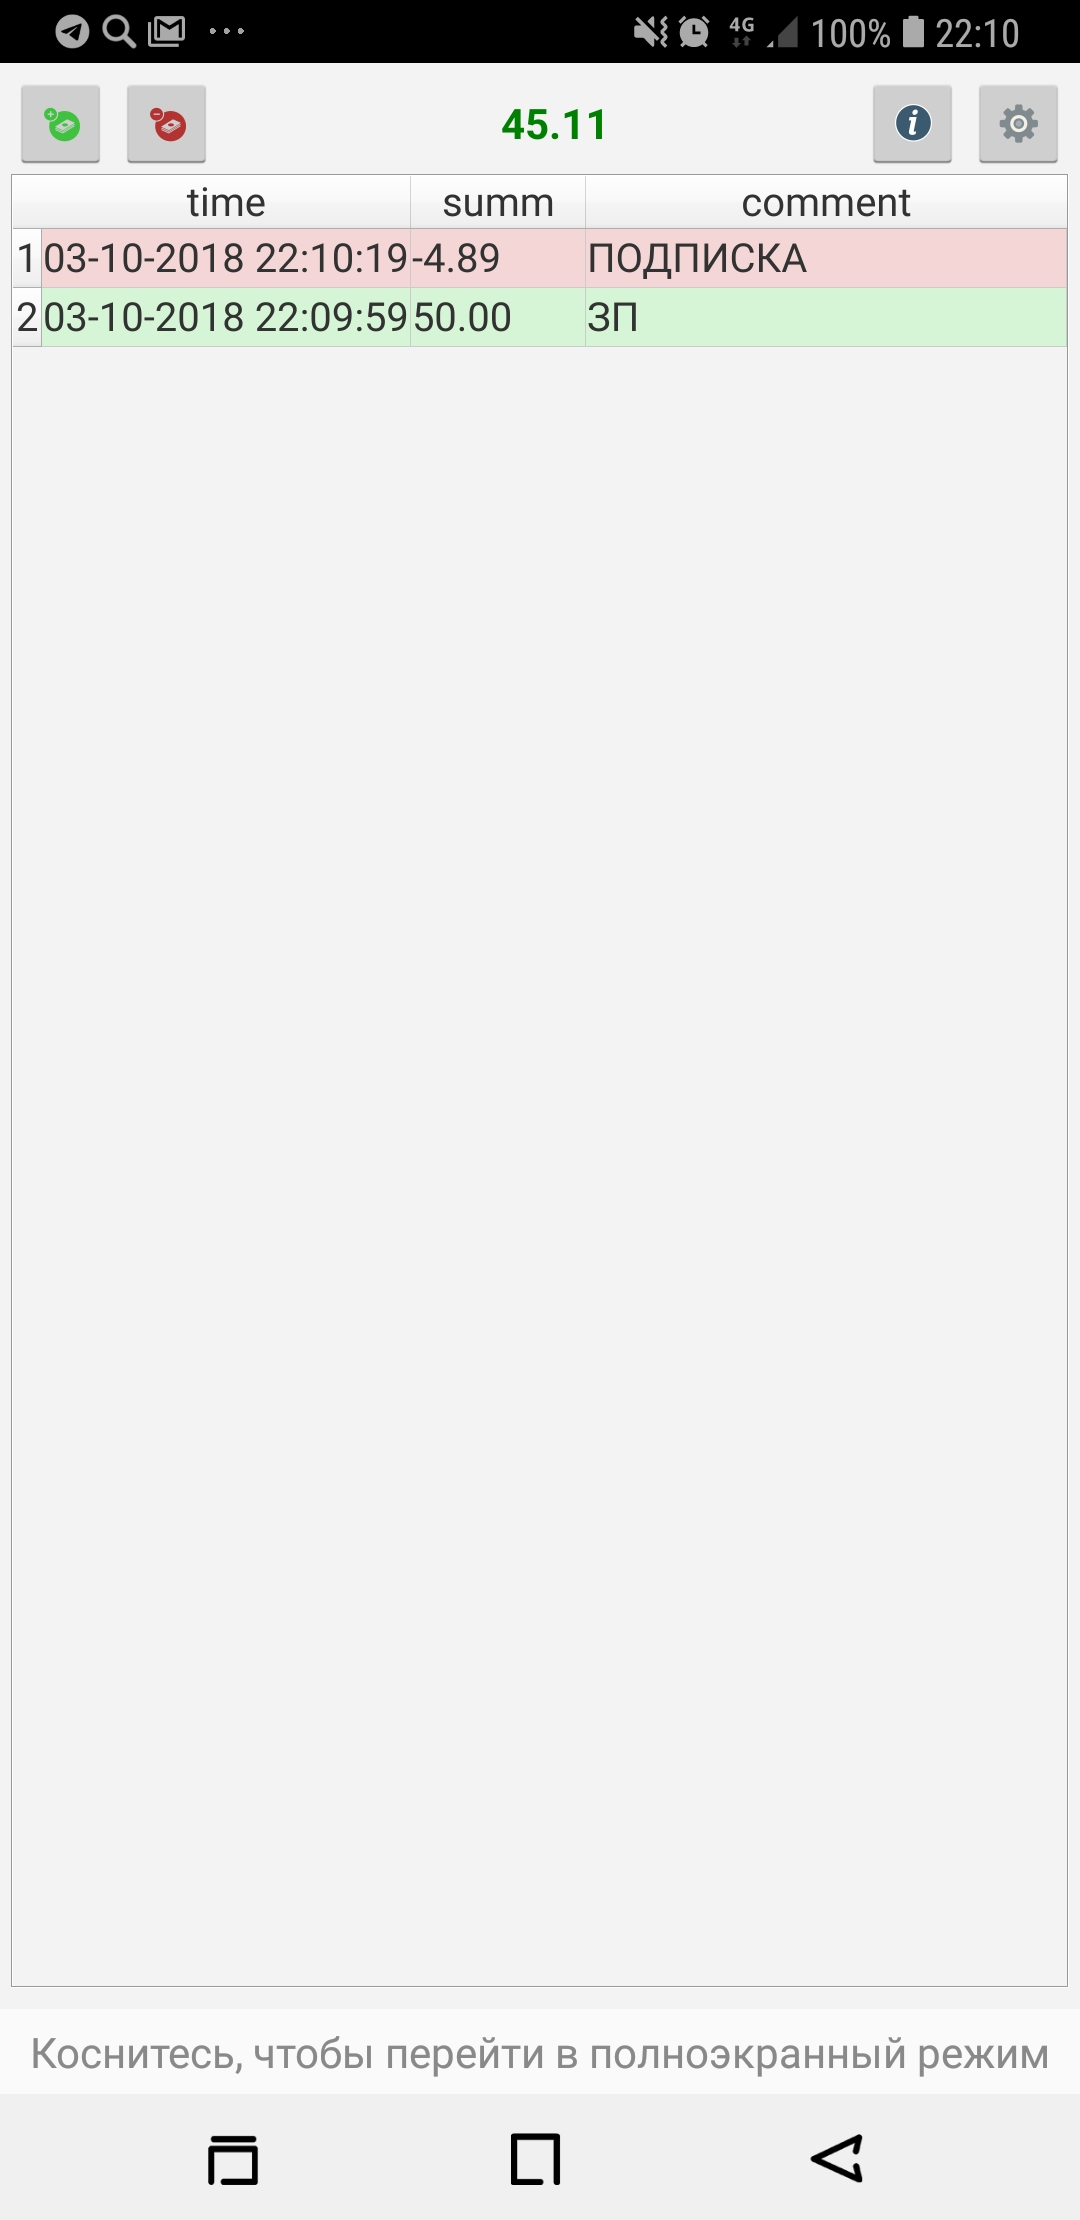
\includegraphics[height=0.7\linewidth]{pics/viewAndroid.eps}
	\caption{Версия для Android}
	\label{fig:viewAndroid}
\end{figure}

